\chapter{Mitgliederverwaltung}\label{einsatz:personal}
Im Kopf des Fensters kann eingestellt werden welche Personen angezeigt werden sollen.
Ebenso kann durch einen Knopfdruck eine E-Mail an alle angezeigten Personen erstellt werden.
Werden bei dieser Aktion Personen gefunden, für die keine Mailadresse angegeben ist,
so können die angegebenen Postadressen in einer CSV-Datei gespeichert werden.
Diese Daten können dann z.B.\ für Serienbriefe genutzt werden.

\section{Einsatzzeiten}\label{einsatz:personal:zeiten}
\begin{figure}[!h]
	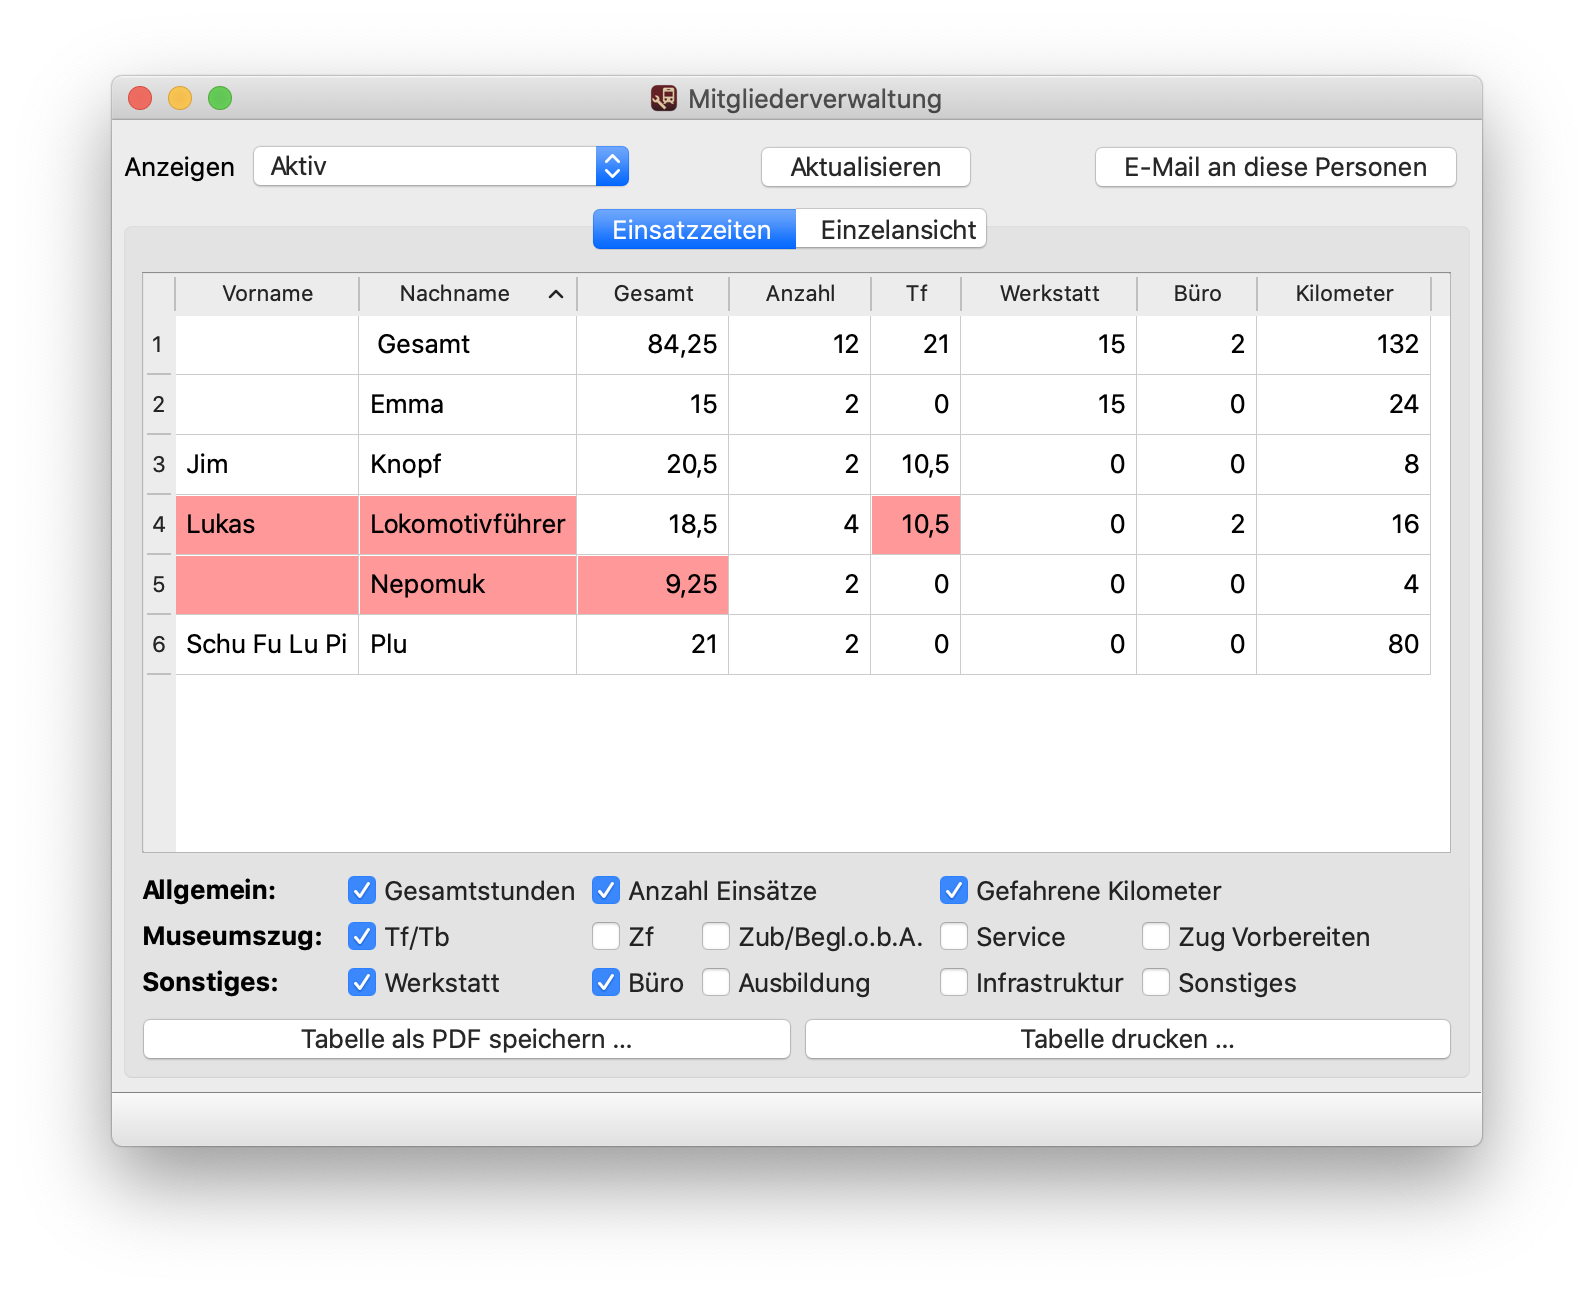
\includegraphics[width=\textwidth]{img/personal_gesamt}
	\caption{Die Mitgliederverwaltung mit den Einsatzzeiten.}
	\label{fig:einsatz:personal:zeiten}
\end{figure}
In der Tabelle von \cref{fig:einsatz:personal:zeiten} wird eine Übersicht über alle in der Kopfzeile ausgewählten Personen gegeben.
Die Einfärbung erfolgt anhand der mindestens zu erbringenden Stunden.
Rot bedeutet hierbei, dass die Person ihre Stunden noch nicht erbracht hat.
Eine weiße Markierung bestätigt, dass die Mindeststunden erbracht wurden, oder keine solchen gefordert sind (z.B.\ bei passiven Mitglieder).
Minderjährige aktive Mitglieder müssen keine Mindeststunden erbringen.
Für aktive Mitglieder gilt, dass sie in die Kategorie "`Aktiv mit Stunden"' fallen, sobald die Mindeststunden für "`Gesamt"' erreicht wurden.
Die persönlichen Mindeststunden (z.B.\ für Lokführer)
werden hierbei nicht berücksichtigt.
Dennoch werden diese Personen auch rot markiert.
Passive Mitglieder, die Stunden geleistet haben, werden grün markiert.
Durch einen Doppelklick auf den Eintrag einer Person in der Tabelle wird die entsprechende Einzelansicht geöffnet.


Mit Hilfe der Auswahlkästchen können die verschiedenen Spalten mit den Zeiten der Personen ein- und ausgeblendet werden, die dann auch entsprechend sortiert werden können.
Ebenso wird die Summe der jeweiligen Spalten in der Zeile "`Gesamt"' angegeben.
Diese Zeile ist in der Ausgabe ebenso enthalten.


Mit den Knöpfen \button{Tabelle als PDF speichern \dots} und \button{Tabelle drucken \dots} kann man die Daten der Tabelle exportieren.
Diese Funktionen sind auch im Menü \button{Exportieren} verfügbar.


\paragraph{Mindeststunden}
Die Mindeststunden können über den Eintrag \aktion{Mindeststunden \dots} im Menü \aktion{Personalmanagement} bearbeitet werden.
Der sich öffnende Dialog ist in \cref{fig:einsatz:personal:mindeststunden} dargestellt.

\begin{figure}[!h]
	\centering
	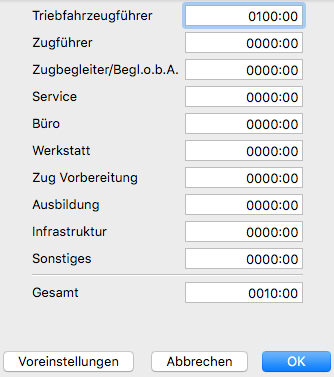
\includegraphics[width=0.5\textwidth]{img/personal_mindeststunden}
	\caption{Der Dialog zum Ändern der Mindeststunden.}
	\label{fig:einsatz:personal:mindeststunden}
\end{figure}

Standardmäßig sind 10 Stunden für alle aktiven Mitglieder eingestellt.
Personal mit Ausbildung zum Lokführer muss 100 Stunden als Lokführer ableisten.
Die Werte für jedes Konto können beliebig geändert werden.

Die Mindeststunden für Ausbildung werden nur für Personal mit einer betrieblichen Ausbildung und bestehender Tauglichkeit angewendet.




\section{Einzelansicht}\label{einsatz:personal:einzelansicht}
\begin{figure}[!h]
	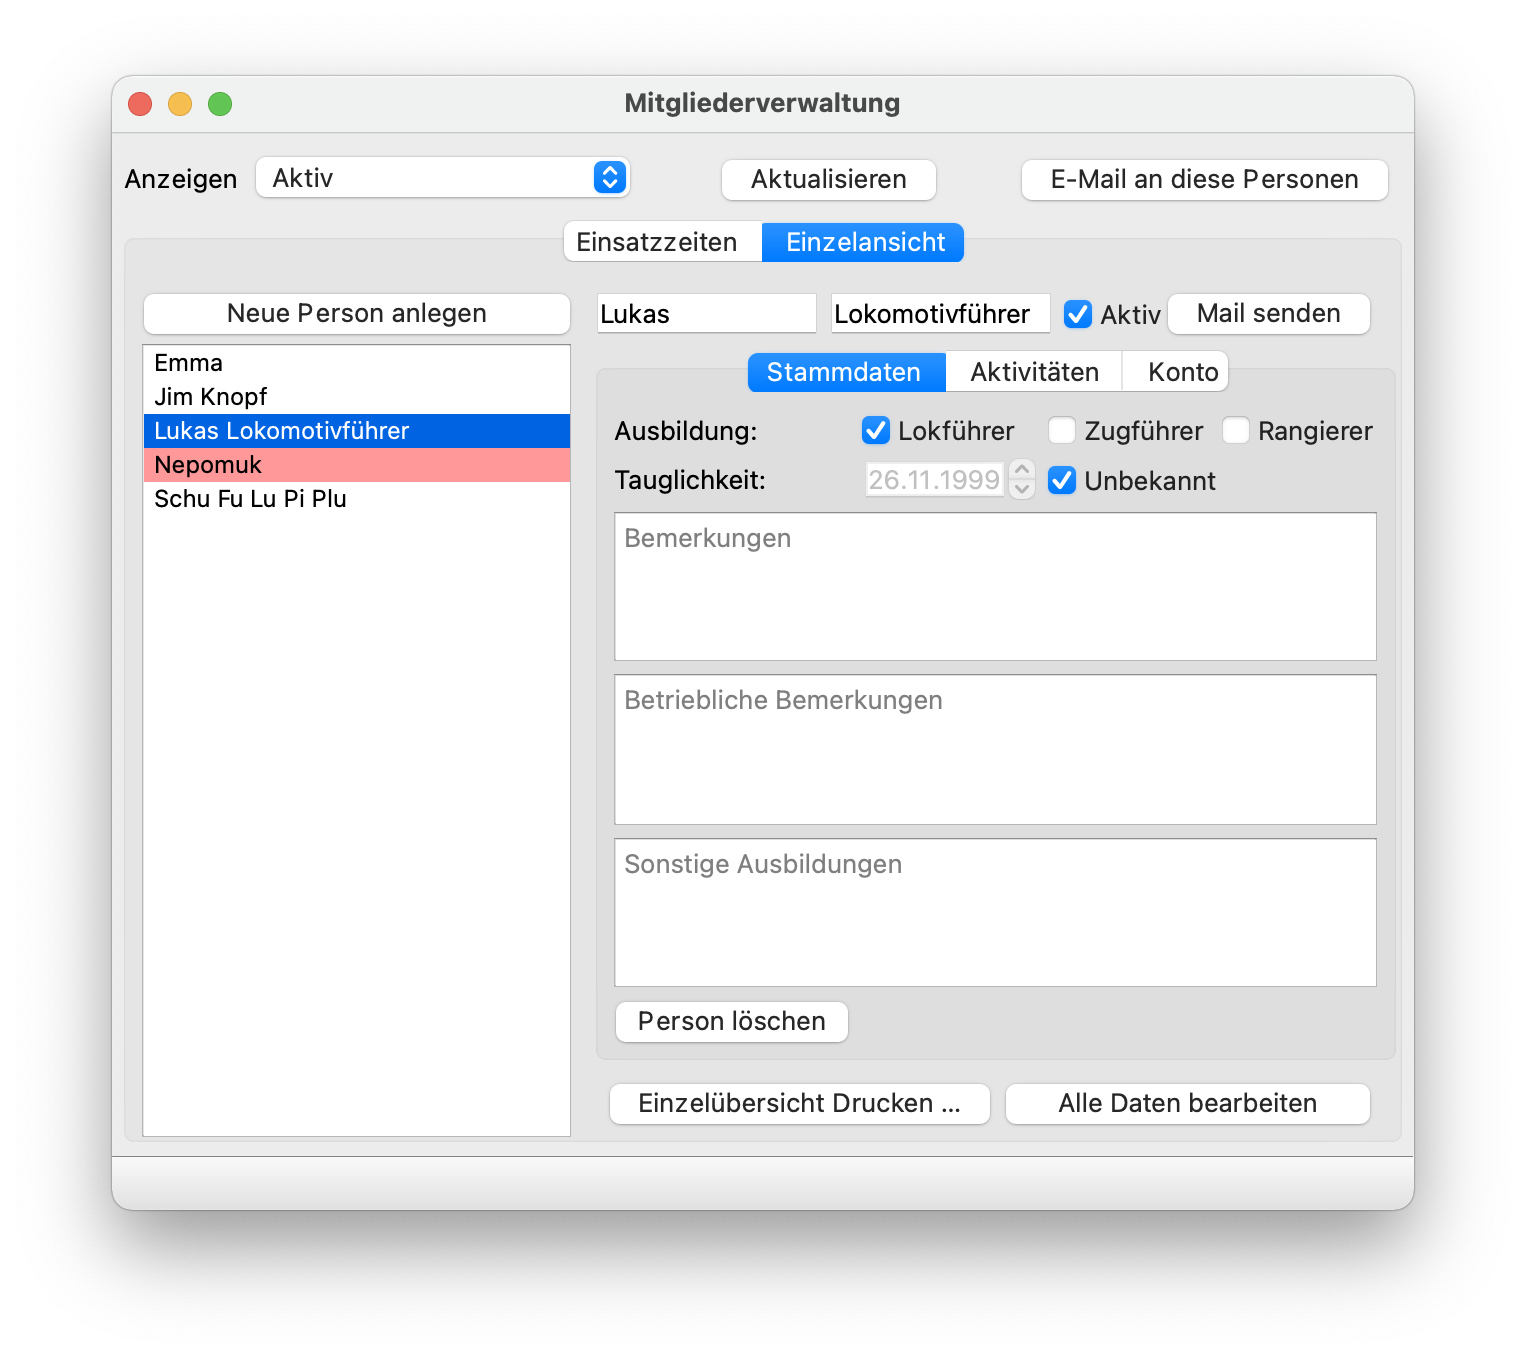
\includegraphics[width=\textwidth]{img/einzelansicht_stammdaten}
	\caption{Die Einzelansicht mit geöffnetem Reiter für die Stammdaten}
	\label{fig:einsatz:personal:einzel:stammdaten}
\end{figure}
Das Fenster mit geöffneter Einzelansicht ist in \cref{fig:einsatz:personal:einzel:stammdaten} zu sehen.
In der Liste sind alle Personen gelistet, die nach der Kopfzeile des Fenster angezeigt werden sollen.
Die farbliche Hervorhebung erfolgt analog zur Gesamtübersicht.
Im oberen Teil können der Name
\begin{neu}
und der Status der Person (aktiv oder passiv) verändert werden.
Ebenso kann per Knopfdruck eine Mail an die Person gesendet werden.
\end{neu}

\begin{neu}
Mit dem Knopf \button{Einzelübersicht drucken \dots} kann die Stundenübersicht der aktuellen Person ausgegeben werden.
\end{neu}
Dort werden dann die Aktivitäten einzeln mit den jeweiligen Zeiten aufgelistet.
Diese Ansicht enthält nur wenige persönliche Informationen.


\paragraph{Stammdaten}
\begin{neu}
Es können nur die betrieblichen Daten und die Bemerkungen bearbeitet werden.
\end{neu}
Über den Knopf \button{Alle Daten bearbeiten} kann der vollständige Datensatz einer Person bearbeitet werden.
Dazu wird das Fenster aus dem \Personal geöffnet.
Siehe \cref{personal:person} für weitere Informationen.
Ebenso kann die Person gelöscht werden.
Allerdings kann die Person auch als ausgetreten markiert werden,
sodass sie nicht gelöscht werden muss.

\hinweis{Eine Person kann erst dann gelöscht werden, wenn Sie in keinen Aktivitäten mehr eingetragen ist.
Siehe nächster Absatz.}


\begin{figure}[!h]
	\centering
	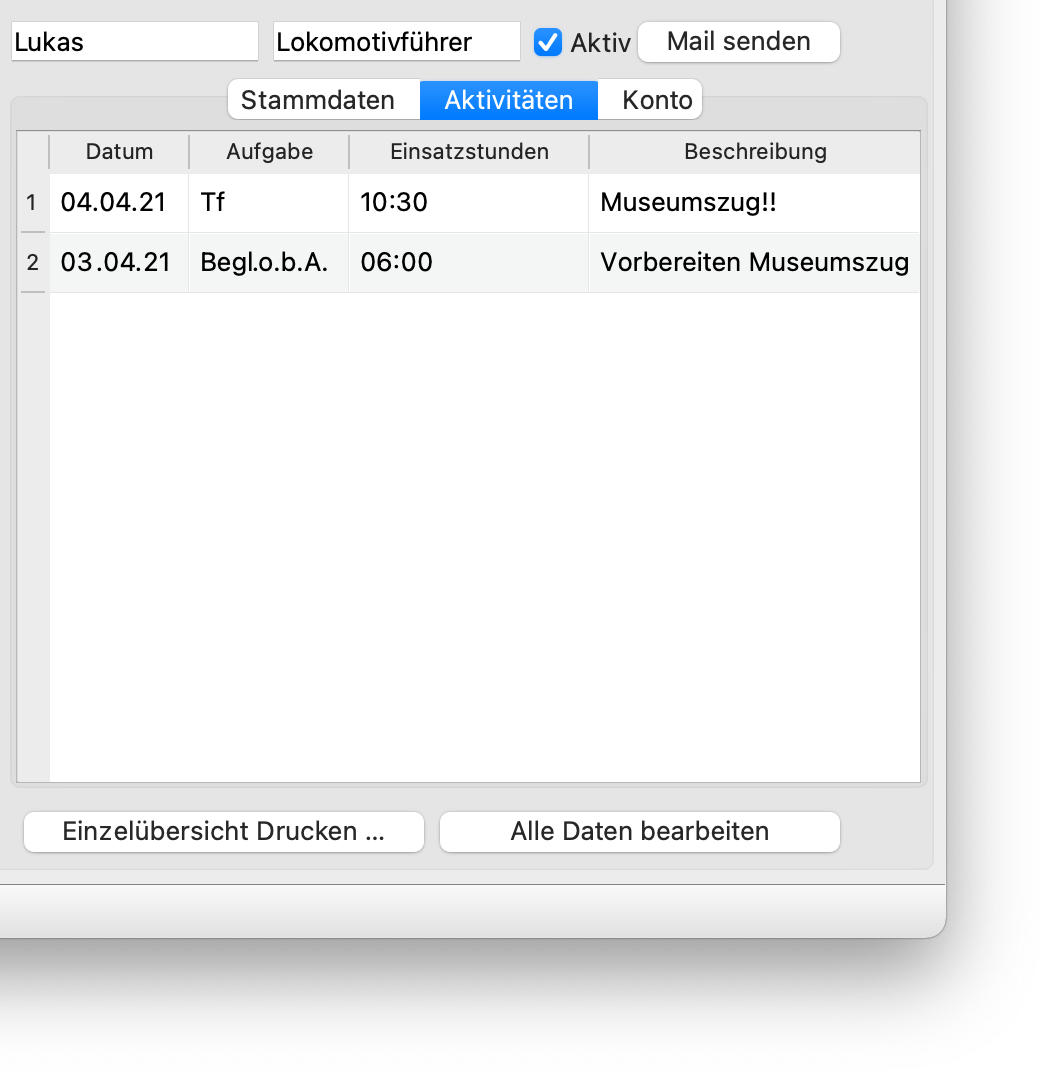
\includegraphics[width=.75\textwidth]{img/einzelansicht_aktivitaeten}
	\caption{Die Einzelansicht mit geöffnetem Reiter für die Aktivitäten}
	\label{fig:einsatz:personal:einzel:aktivitaeten}
\end{figure}
\paragraph{Aktivitäten}
Der Reiter,
des in \cref{fig:einsatz:personal:einzel:aktivitaeten} dargestellten Fensters,
zeigt eine Tabelle mit den Aktivitäten,
an denen die ausgewählte Person mitgeholfen hat.


\begin{figure}[!h]
	\centering
	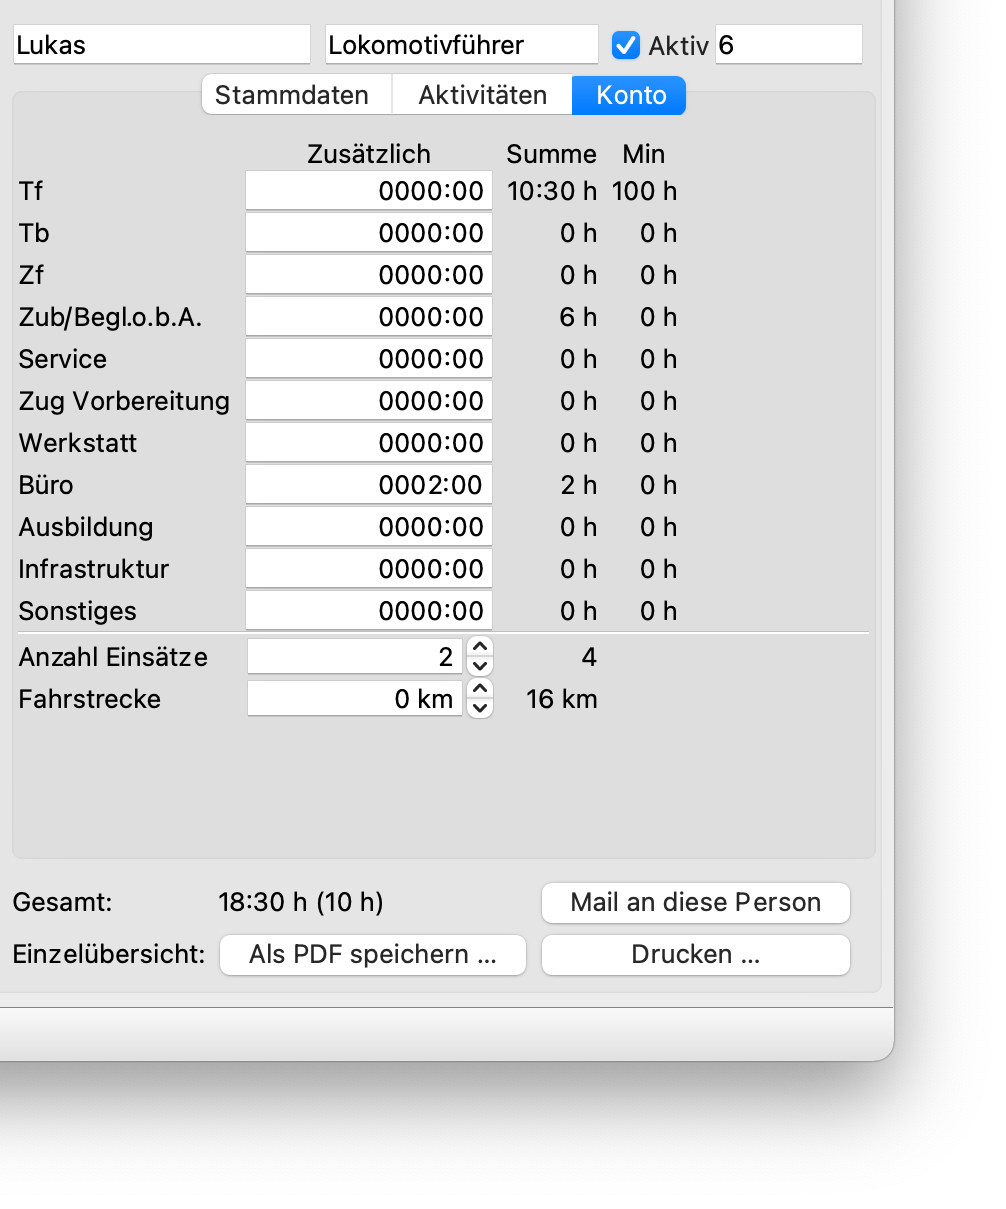
\includegraphics[width=.75\textwidth]{img/einzelansicht_konto}
	\caption{Die Einzelansicht mit geöffnetem Reiter für das Zeitenkonto}
	\label{fig:einsatz:personal:einzel:konto}
\end{figure}
\paragraph{Konto}
Die Übersicht in \cref{fig:einsatz:personal:einzel:konto} enthält die Zeiten aufgeteilt nach den verschiedenen Zeit-Konten.
Ebenso können hier zusätzliche Stunden und Kilometer eintragen werden,
welche die Person geleistet hat, aber keiner im System erfassten Aktivität zuzuordnen sind.
Die Anzahl der zusätzlichen Aktivitäten kann ebenfalls erfasst werden.
Ebenso kann man sehen, in welchen Gebieten die Person ihre Pflichtstunden erfüllt hat und wieviele Mindeststunden Sie jeweils in den Gebieten erbringen muss.

\begin{hinweis}
  Für alle Darstellungen und Berechnungen werden nur die Zeiten angerechnet, die bisher auch wirklich abgeleistet wurden,
  also deren Datum in der Vergangenheit lag.
\end{hinweis}



\section{Exportfunktionen}
Es stehen folgende Möglichkeiten zur Verfügung,
die alle über das Menü \aktion{Exportieren} im Fenster des Mitgliederverwaltung aufgerufen werden können:
\begin{description}
  \item[Einzelansicht(en)]
  Das ausgegebene Dokument enthält die Aktivitäten, die Einsatzzeiten und Mindeststunden für die jeweilige Person.
  Ebenso wird die betriebliche Ausbildung (sofern vorhanden und Tauglichkeit gegeben) und die Entfernung zum Bahnhof angegeben.

  Alle Übersichten werden in einer Datei zusammengefasst.
  Wenn \enquote{für alle} gewählt wurde,
  wird das Dokument um eine Übersicht ergänzt,
  welche die Summe aller geleisteten Stunden umfasst.
  Dort sind auch die Mindeststunden der einzelnen Kategorien angegeben.

  \item[Tabelle Einsatzzeiten]
  Alle in der Tabelle angezeigten Informationen werden in der angegebenen Sortierung ausgegeben.
  Diese Ausgabemöglichkeit ist auch über die zwei Knöpfe in der Gesamtübersicht verfügbar.

  \item[Personalblatt]
  Die Personalblätter enthalten für jede Person alle personenbezogene Daten,
  die im Programm verwaltet werden.
  Einsatzzeiten und geleistete Stunden sind in diesen Ansichten nicht enthalten.

  \item[Mitgliederliste]
  In dieser Liste sind alle Personen enthalten, die aktuell in der Liste angezeigt werden.
  Ausgegeben werden dabei alle personenbezogenen Daten,
  die im Programm verwaltet werden.
  Einsatzzeiten und geleistete Stunden sind in diesen Ansichten nicht enthalten.

  \item[Beiträge]
  \begin{neu}
  Hier können CSV-Dateien für den Beitragseinzug erstellt werden.
  Zum einen kann der reguläre Beitrag eingezogen werden (jährlich).
  Zum anderen kann auch der Betrag für Nachzahlungen exportiert werden.
  Dies ist zum Beispiel für Mitglieder relevant,
  die ihre Pflichtstunden nicht erbracht haben
  und somit einen höheren Beitrag zahlen müssen.
  \end{neu}
\end{description}
